\documentclass{article}



ewe

\usepackage{graphicx} % Required for inserting images
\usepackage{amsmath} % Required for some math elements
\usepackage{mathtools} % Required for some math elements

\title{SE vacuum stability}
\author{Orr David}
\date{June 2024}

\begin{document}

\maketitle

\section{Introduction}
\subsection{The unperturbed solution}
here some historic background on the SE\\
the equations describing the problem

\subsubsection{The self-similar solution}
The Euler fluid dynamics equations describe the motion of an inviscid fluid. in a spherically symmetric density profile $\rho = \kappa r^{-\omega}$, the equations are given by

\begin{align}
    \begin{split}
        0	&=\left(\partial_{t}+u\partial_{r}\right)\rho+\frac{\rho}{r^{2}}\frac{\partial}{\partial r}\left(r^{2}u\right)\\
        0	&=\rho\left(\partial_{t}+u\partial_{r}\right)u+\partial_{r}\left(\frac{\rho c^{2}}{\gamma}\right)\\
        0	&=\left(\partial_{t}+u\partial_{r}\right)\left(\frac{c^{2}\rho^{1-\gamma}}{\gamma}\right)            
    \end{split}
\end{align}


We predict that at large $t$ the solution is self-similar, so the variables can be written as -
\begin{align}
    \begin{split}
        \xi &\equiv \frac{r}{R\left(t\right)}\\
        u\left(r,t\right)	=\dot{R}\xi U\left(\xi\right) \quad \quad
        c\left(r,t\right)	&=\dot{R}\xi C\left(\xi\right) \quad \quad
        \rho\left(r,t\right)	=BR^{\varepsilon}G\left(\xi\right)
    \end{split}
\end{align}
And by inserting these into the equations we get the following ODEs -
\begin{align}
    \begin{split}
        0 &= \left[\varepsilon-\xi\left(\log\left(G\right)'\right)\right]+\xi U\left(\log\left(G\right)'\right)+\left(\xi U\right)'+2U	\\
        0 &= \left[\delta\xi U+\xi\left(U-1\right)\left(\xi U\right)'\right]+\frac{1}{\gamma G}\left(G\xi^{2}C^{2}\right)'	\\
        0 &= 2\delta-\left(\gamma-1\right)\varepsilon+\xi\left(U-1\right)\left[\log\left(\xi^{2}C^{2}\right)-\left(\gamma-1\right)\log\left(G\right)\right]'
    \end{split}
\end{align}
Where $\delta = \frac{R\ddot{R}}{\dot{R}^{2}}$.\\
In order to get a self-similar time-independent solution, we demand that $\delta = const$. 
In the shock front we have the boundary conditions from the Rankine-Hugoniot conditions -

\begin{align}
    \begin{split}
        G\left(1\right)	=\frac{\gamma+1}{\gamma-1} \quad \quad
        C\left(1\right)	=\frac{\sqrt{2\gamma\left(\gamma-1\right)}}{\gamma+1} \quad \quad
        U\left(1\right)	=\frac{2}{\gamma+1}
    \end{split}
\end{align}

Using the boundary conditions we can calculate the value of $\varepsilon = - \omega$ in order for the the two sides of the shock to scale correctly.\\


The PDE can be better understood by rewriting it by the following variables - 
\begin{align}
    \label{eq:charcteristics}
    \begin{split}
        \Delta &= C^{2} - (1-U)^{2} \\
        \Delta_{1} &= U(1-U)(1-U-\delta) - C^{2}(3U + \frac{\varepsilon+2\delta}{\gamma}) \\
        \Delta_{2} &= C(1-U)(1-U-\delta) - \frac{\gamma-1}{2}CU(2-2U+\delta) - C^{2} + \frac{2\delta-(\gamma-1)\varepsilon}{2\gamma}\frac{C^{3}}{1-U}
    \end{split}
\end{align}
And the equation is reduced to following -
\begin{align}
    \begin{split}
        \frac{dU}{d\log\xi} = \frac{\Delta_{1}}{\Delta} \quad \quad
        \frac{dC}{d\log\xi} = \frac{\Delta_{2}}{\Delta}
    \end{split}
\end{align}
and $G$ is given by the following - 
\begin{align}
    \label{eq:G_(U,C)}
    \begin{split} 
    G &=\sqrt[\gamma-1+\lambda]{\kappa\cdot C^{2}\cdot\xi^{2-3\lambda}\left(1-U\right)^{-\lambda}}\\
    \lambda &=\frac{2\delta+\omega\left(\gamma-1\right)}{3-\omega}
    \end{split}
\end{align}
\subsubsection{The first type solutions}
The first type solutions where discovered by Taylor, Seydov, and Von-Neumann. 
By taking $\delta = \frac{\omega - 3}{2}$ we can solve the equations.\\
It is important to note that for $\omega \in \left(2,3\right)$ we get a "vacuum" solution, we shall return to this later.\\
\subsubsection{The second type solutions}
The second type solutions where\dots
 
\subsubsection{third type solutions}
here some background on the third type solutions, including the work by Gruzinov.

\begin{figure}
    \centering
    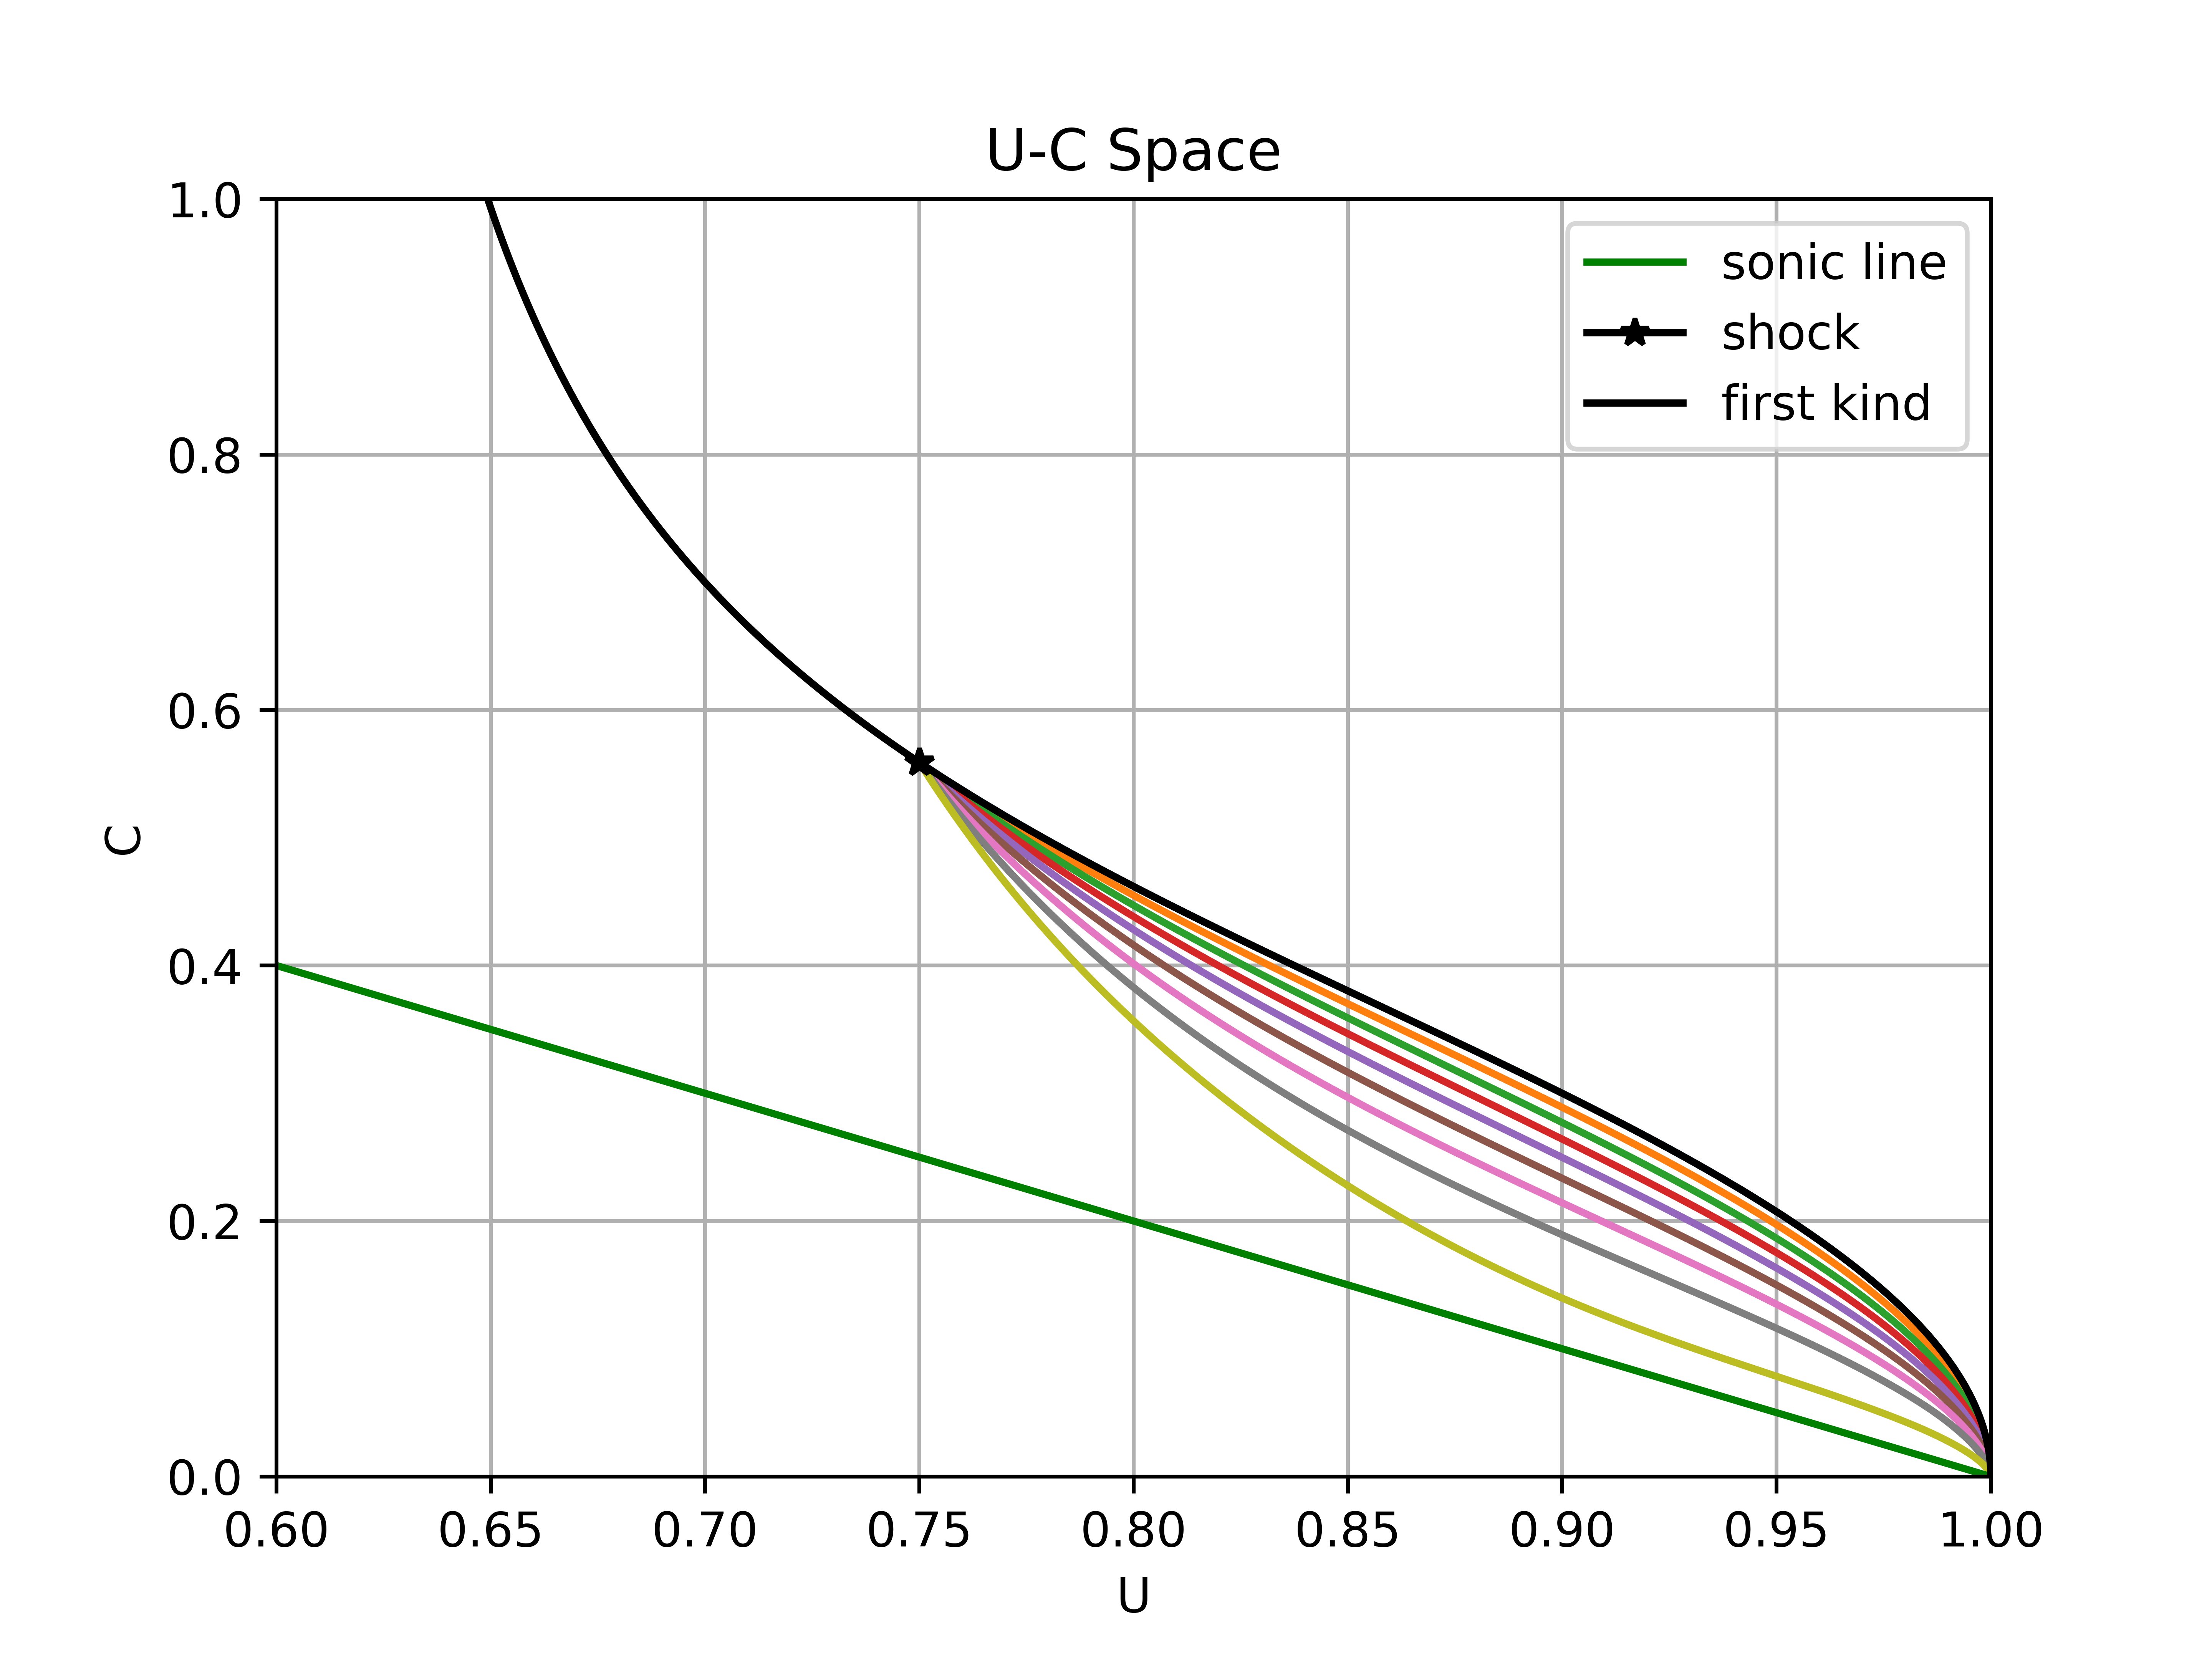
\includegraphics[width=1\linewidth]{3rd_type_solutions.png}
    \caption{Enter Caption}
    \label{fig:enter-label}
\end{figure}


\subsubsection{The vacuum solution}
Once the solution reaches $U=1$, 
in which cases we have a vacuum in our solution
\begin{figure}
    \centering
    \includegraphics[width=1\linewidth]{last_xi.png}
    \caption{Enter Caption}
    \label{fig:enter-label}
\end{figure}


\subsection{The perturbed solution}
here some background on the perturbation, including the work by Ream, waxman, j sanz...

\subsubsection{the methods used}
Let the perturbed variables be given by the following -
\begin{align}
    \begin{split}
        \delta\vec{v} &= \vec{v}\left(r,\theta,\phi,t\right) - v_{0}\left(r,t\right) \\
        \delta p &= p\left(r,\theta,\phi,t\right) - p_{0}\left(r,t\right) \\
        \delta\rho &= \rho\left(r,\theta,\phi,t\right) - \rho_{0}\left(r,t\right)        
    \end{split}
\end{align}
And by separtion of variables we get the following equations -
\begin{align}
    \begin{split}
        \delta\vec{v}\left(r,\theta,\phi,t\right) &= \xi\dot{R}\left[\delta U_{r}\left(\xi\right)Y_{lm}\left(\theta,\phi\right)\hat{r}+\delta U_{T}\left(\xi\right)\nabla_{T}Y_{lm}\left(\theta,\phi\right)\right]f\\
        \delta\rho\left(r,\theta,\phi,t\right)&=BR^{\varepsilon}\delta G\left(\xi\right)Y_{lm}\left(\theta,\phi\right)f\\
        \delta p\left(r,\theta,\phi,t\right)&=BR^{\varepsilon}\delta G\left(\xi\right)Y_{lm}\left(\theta,\phi\right)f            
    \end{split}
\end{align}
after inserting these into the equations and taking only first derivatives of the perturbed variables we get the following equations -
\begin{align}
    0 &= \frac{\partial\delta\rho}{\partial t}+r^{-2}\frac{\partial}{\partial r}\left(r^{2}v_{0}\delta\rho\right)+\nabla\left(\rho_{0}\delta\vec{v}\right)\\
    0 &= \frac{\partial\delta\vec{v}}{\partial t}+v_{0}\frac{\partial\delta\vec{v}}{\partial r}+\delta v_{r}\frac{\partial v_{0}}{\partial r}\hat{r}-\rho_{0}^{-2}\frac{\partial p_{0}}{\partial r}+\rho_{0}^{-1}\nabla\left(\delta p\right)+r^{-1}v_{0}\delta v_{t}\\
    0 &= \left(\frac{\partial}{\partial t}+v_{0}\frac{\partial}{\partial r}\right)\left(\frac{\delta p}{p_{0}}-\gamma\frac{\delta\rho}{\rho_{0}}\right)+\delta v_{r}\left(p_{0}^{-1}\frac{\partial p_{0}}{\partial r}-\gamma\rho_{0}^{-1}\frac{\partial\rho_{0}}{\partial r}\right)
\end{align}
Or in matrix form -
\begin{align}
    MY'=NY
\end{align}
where 
\begin{align}
    Y=\begin{bmatrix}\delta G\\
        \delta U_{R}\\
        \delta U_{T}\\
        \delta P
        \end{bmatrix}
        \quad q=\frac{\dot{f}R}{f\dot{R}}
\end{align}
\begin{align}
    M&=\begin{bmatrix}\xi\left(U-1\right) & G\xi & 0 & 0\\
        0 & \left(U-1\right)\xi^{2}G & 0 & 1\\
        0 & 0 & \left(U-1\right)\xi^{2}G & 0\\
        -\frac{\gamma\xi}{G}\left(U-1\right) & 0 & 0 & \frac{\xi}{P}\left(U-1\right)
        \end{bmatrix}\\
    N&=\begin{bmatrix}\omega-q-3U-\xi U' & -\xi G'-3G & l\left(l+1\right)G & 0\\
        P'G^{-1} & \left(1-\delta-q-2U-\xi U'\right)G\xi & 0 & 0\\
        0 & 0 & \left(1-\delta-q-2U\right)G\xi & -\xi^{-1}\\
        \frac{\gamma q}{G}-\xi\gamma\left(U-1\right)\frac{G'}{G^{2}} & \xi\gamma\frac{G'}{G} & 0 & \xi\left(U-1\right)\frac{P'}{P^{2}}-\frac{q}{p}
        \end{bmatrix}
\end{align}
And the boundary conditions in the shock front are given by the following -
\begin{align}
    \begin{split}
        \delta G\left(1\right)&=-\frac{\gamma+1}{\gamma-1}\omega-G'\\
        \delta U_{r}\left(1\right)&=\frac{2}{\gamma+1}q-U'\\
        \delta U_{T}\left(1\right)&=-\frac{2}{\gamma+1}\\
        \delta P\left(1\right)&=\frac{2}{\gamma+1}\left[2\left(q+1\right)-\omega\right]-P'
    \end{split}
\end{align}

Now, the way to solve this is by integrating the equations from the shock front to the singular point. only for correct values of $q$ we will get a solution that doesn't diverge at the singular point.\\
This method works very well for the second type solutions, but for the third type solutions we encounter a problem, as the base solution diverges at the singular point.

\subsubsection{The perturbed solution for the second type solutions}


\subsection{Analyzing the singular point in solutions with a vacuum}
Near the singular point $C \rightarrow 0$, $U \rightarrow 1$, and $G \rightarrow \infty$.\\
we will denote $U$ as a function of $C$ - 
\begin{align}
    \left(U - 1\right) &= A C^{\theta}
\end{align}
and by inserting this into the equation  and we get the following -
\begin{align}
    \theta \left( 3\leq \delta \leq 3.26 \right) &=\frac{6\gamma - 2\omega}{\left(\gamma-1\right)\omega} \in \left( 1,2 \right)\\
    \theta \left( 2 \leq \delta \leq 3 \right) &= 2\\
    A &= const\dots
\end{align}
And the other variables are - 
\begin{align}
    G &= G_{0}\cdot C^{-2}\cdot\xi_{vacuum}^{3-2\omega}\\
    P &= \frac{G_{0}}{\gamma}\cdot\xi_{vacuum}^{5-2\omega}\\
    G_{0} &= const\dots
\end{align}
In order to understand what the perturbations look like near the singular point, we will look at the possible eigenvalues of equation - 
\begin{align}
    \det \left( M - \lambda N \right) &= 0
\end{align}
the matrix is then - 
\begin{align*}
    \begin{bsmallmatrix}-\xi AC^{\theta}-\lambda\left[\omega\left(1-\frac{\xi}{5}\right)+3\left(\xi-1\right)-q\right] & \gamma P\xi^{-1}\cdot C^{-2}-\lambda\gamma P\frac{2\omega}{5A}\xi^{-1}C^{-2-\theta} & -\lambda\gamma P\cdot l\left(l+1\right)\xi^{-2}C^{-2} & 0\\
        -\lambda\left[3-\frac{6}{5}\omega\right]\xi\cdot C^{2} & -A\gamma PC^{\theta-2}-\lambda\gamma P\left(3\xi\left(1-\frac{\omega}{5}\right)-\left(1+q\right)\right)\xi^{-1}C^{-2} & 0 & 1\\
        0 & 0 & -A\gamma PC^{\theta-2}+\lambda\gamma P\left(1+q\right)\xi^{-1}C^{-2} & \lambda\xi^{-1}\\
        \frac{A}{P}\xi^{3}C^{\theta+2}-\frac{\lambda}{P}\left[q-2\xi\frac{\omega}{5}\right]\xi^{2}C^{2} & \lambda\gamma\xi\frac{2\omega}{5A}C^{-\theta} & 0 & -\frac{A}{P}\xi C^{\theta}+\lambda\frac{q}{P}
    \end{bsmallmatrix}
\end{align*}
and the determinant is -
\begin{multline*}
    0=\left[-\xi AC^{\theta}-\lambda\left[\omega\left(1-\frac{\xi}{5}\right)+3\left(\xi-1\right)-q\right]\right] \\
    \times \left[\gamma^{2}PC^{-2}\left[\left(C^{-2}\left(\lambda\left(1+q\right)\xi^{-1}-AC^{\theta}-\lambda3\left(1-\frac{\omega}{5}\right)\right)\right.\right.\right. \right. \\
    \left.\left.\left.\left(\lambda q-A\xi C^{\theta}\right)-\lambda\xi\frac{2\omega}{5A}C^{-\theta}\right)\left(\lambda\left(1+q\right)\xi^{-1}-AC^{\theta}\right)\right]\right] \\
    +\lambda\left[3-\frac{6}{5}\omega\right]\gamma^{2}P\left(\left(1-\lambda\frac{2\omega}{5A}C^{-\theta}\right)\left(\lambda\left(1+q\right)\xi^{-1}-AC^{\theta}\right)\right. \\
    \left.\left.\left(\lambda q-A\xi C^{\theta}\right)C^{-2}-\lambda^{3}\frac{2\omega}{5A}C^{-\theta}\xi^{-1}l\left(l+1\right)\right)-\xi\left[A\xi C^{\theta}-\lambda\left[q-2\xi\frac{\omega}{5}\right]\right] \\
    \times \left[\gamma^{2}P\cdot\left[\left(AC^{\theta}+\lambda\left(3\xi\left(1-\frac{\omega}{5}\right)-\left(1+q\right)\right)\xi^{-1}\right)\right.\right.\right. \\
    \left.\left.\left.\left.\left(l\left(l+1\right)C^{-2}\right)\lambda^{2}\xi^{-2}+\left(AC^{\theta-2}-\lambda\left(1+q\right)\xi^{-1}C^{-2}\right)\left(1-\lambda\frac{2\omega}{5A}C^{-\theta}\right)\right]\right]\right]
\end{multline*}

\subsubsection{finding the eigenvalues}
in order to find the eigenvalues we will assume that $\lambda$ is a function of $C$, so $\lambda = \lambda_0 C^{\alpha}$.\\ 
Let us divide and conquer,
\begin{enumerate}
    \item if $\alpha > \theta$ then we get that near the singular point $\alpha = \theta - 2$ and thus a contradiction.
    \item if $\alpha = \theta$ then we get the following eigenvalues -
    \begin{align}
        \lambda_0 &= \frac{A\xi}{q}\\
        \lambda_0 &=\frac{A\xi}{q + 1 - 3 \xi \left(1-\frac{\omega}{5}\right)}\\
        \lambda_0 &=\frac{A\xi}{q + \omega\left(\frac{\xi}{5} - 1\right)+3\left(1 - \xi\right)}
    \end{align}
    \item if $\theta - 2 < \alpha < \theta$ - then the determinant is given by -
    \begin{equation*}
        0=\lambda_0^{3}C^{3\alpha-4}\left[\omega\left(1-\frac{\xi}{5}\right)+3\left(\xi-1\right)-q\right]\left[\left(1+q\right)\xi^{-1}-3\left(1-\frac{\omega}{5}\right)\right]q
    \end{equation*}
    it means that in order to get non zero eigenvalues the values of $q$ have to be one of the following - 
    \begin{align}
        \begin{split}
            q_1&=0\\
            q_2&=\omega-\xi_{vacuum}\left(\frac{\omega}{5}+3\right)-3<0\\
            q_3&=\xi_{vacuum}\left(3-\frac{3}{5}\omega\right)-1>0
        \end{split}
    \end{align}
    which is weird, because it is independent of $l$.
    \item if $\theta - 2 = \alpha$ - then we get the following eigenvalue - 
    \begin{equation}
        \lambda_0=\frac{\left[\omega\left(1-\frac{\xi}{5}\right)+3\left(\xi-1\right)-q\right]\left[\left(1+q\right)\xi^{-1}-3\left(1-\frac{\omega}{5}\right)\right]}{\left[3-\frac{6}{5}\omega\right]\frac{2\omega}{5A}\left(1+q\right)\xi^{-1}}
    \end{equation}
    this seams to be the only option to get an eigenvalue where the perturbations don't diverge more then the base solution as we approch the singular point.
    \item if $\theta - 2 > \alpha$ - then we get the following determinant -
    \begin{equation*}
        0=\lambda_0^{4}C^{\alpha-\theta}\left[3-\frac{6}{5}\omega\right]\frac{2\omega}{5A}\left(q\left(1+q\right)\xi^{-1}\right)
    \end{equation*}
    meaning that in order to get any non-zero eigenvalues the values of $q$ have to be $q = -1,0$
\end{enumerate}

\section{The vacuum stability}
\subsection{the approximations near the singular point}






\end{document}
